\title{\bf Lecture 3 Review - Centralized and Decentralized Cryptocurrencies\\}
\author{\bf Rylan Schaeffer and Vincent Yang\\}
\date{\bf \today \\}

\documentclass{article}
\renewcommand{\thesubsection}{\thesection.\alph{subsection}}
\usepackage{enumerate}
\usepackage{hyperref}
\usepackage{amsmath}
\usepackage{graphicx}
\setlength{\oddsidemargin}{0in}
\setlength{\evensidemargin}{0in}
\setlength{\textheight}{9in}
\setlength{\textwidth}{6.5in}
\setlength{\topmargin}{-0.5in}

\begin{document}
\maketitle

Note: This lecture is based on Princeton University's BTC-Tech: Bitcoin and Cryptocurrency Technologies Spring 2015 course.

\section*{Agenda}
\begin{itemize}
  \item Final Project
    \subitem Rudimentary cryptocurrency
    \subitem Groups vs. Pairs vs. Single
    \subitem Report on some study/article about Bitcoin/Cryptocurrencies
    \subitem Other ideas
  \item Homework 3
  \item Lecture Review/Clarification
    \subitem Why decentralize?
    \subitem Problems to solve/How proof of work solves them
    \subitem Mining/Motivations/Why it's important (Proof of work)
    \subitem Shortest vs. Longest blockchain
    \subitem Double spending
    \subitem 51\% attacker
\end{itemize}

\section*{Advantages to Centralization}
\begin{itemize}
  \item Automation:
    \subitem Easily manage a large number of keys e.g. Mastercard Europe
    \subitem Maintain secure infrastructure and improve operations/efficiency
  \item Centralized Monitoring:
    \subitem Record everything that happens easily; brings transparency
  \item Centralized Policy
  \item Easily update and track keys
  \item Easily update cryptographic schemes - swap out algorithms
\end{itemize}

\section*{CentralizedCoin}

\section*{Decentralized Cryptocurrencies}
\begin{itemize}
  \item How does Bitcoin deal with Decentralization?
    \subitem Problems to address, since it's no longer centralized
    \begin{enumerate}
      \item Who maintains ledger of transactions?
      \item Who determines which transactions are valid/invalid?
      \item Who creates new coins
      \item Who chooses when rules change
    \end{enumerate}
\end{itemize}

\section*{Distributed Consensus (Solves 1 and 2)}
\begin{center}
  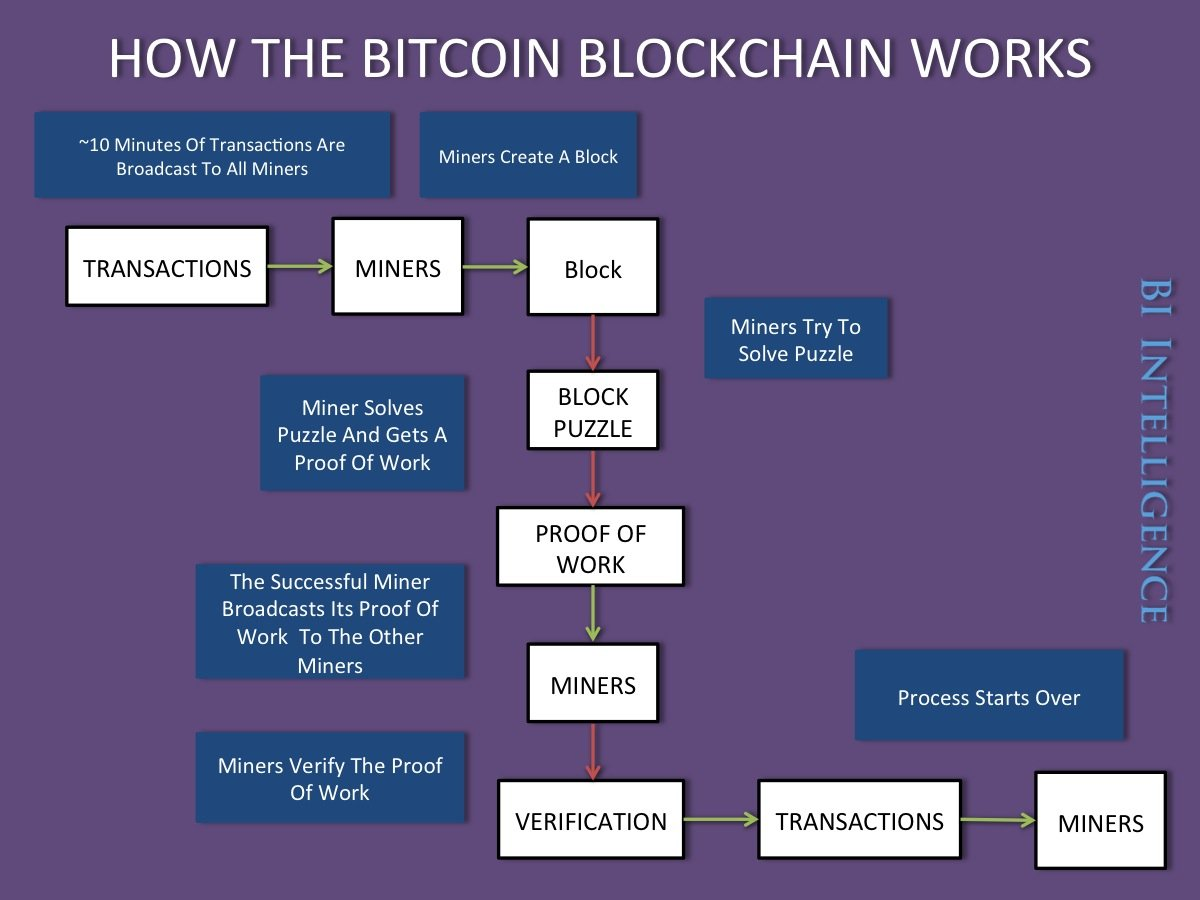
\includegraphics[width=10cm, height=6cm]{process.jpg}
\end{center}
\section*{Block}
\begin{center}
  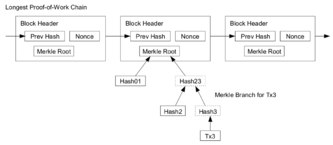
\includegraphics[width=10cm, height=6cm]{merkle.png}
\end{center}
The public ledger (block chain) was started on Jan 3, 2009 presumably by Satoshi Nakamoto. The first
block is called the Genesis Block. This is a special case in the source code.
\section*{Proof of work:}
\begin{itemize}
  \item Puzzle Friendliness: No solving strategy for finding $H(k | x)=y$ is better than trying random values of x.
  \item Select nodes in proportion to computational power
  \item \emph{Give example of leading 0's}
  \item Difficult to compute
  \item Motivation to subvert the process (picking a hopefully honest node), so reward honest nodes
  \item Use bitcoins to incentivize honest nodes - mining. Reward only if it becomes legitimate transaction
  \item Every 210,000 blocks (4 years), block reward is cut in half. Geometric sum - 21 million bitcoins
  \item Nonce published as part of the block.
  \item Proof of work details
    \begin{itemize}
      \item Mining: Hash function with nonce appended to beginning (ex: 0's)
      \item HashCash - with SHA-256 (used twice)
      \item Less than some value
      \item Items used: version, prevBlockHash, merkleRoot, timestamp, bits, nonce
      \item Selecting nodes based on processing power/proportional
      \item Hash puzzles - to make blocks, it needs to find a nonce where
      \item $ H(nonce\ ||\ prev\_hash\ ||\ tx\ ||\ tx\ ||\ ...\ ||\ tx)\ <\ target $
      \item Nonce: Random number that is only used once
      \item Hash puzzle properties: difficult, parameterizable cost (10 minutes variable target), trivial to verify
      \item 10 minutes: reduce inefficiency from having many blocks
      \item $ mean time to next block = \frac{10 minutes}{fraction\ of\ hash\ power} $
      \item proof of stake - proportion to ownership of currency (used in other cryptocurrencies)
      \item http://www.righto.com/2014/09/mining-bitcoin-with-pencil-and-paper.html
    \end{itemize}
  \item Difficulty: what network hash rate results in a given difficulty?
    \subitem Currently, the entire network of miners makes about 30 trillion attempts a second.
    \subitem Difficulty is adjusted every 2016 blocks based on the time it took to find them.
    \subitem At the desired rate of one block every 10 minutes, 2016 blocks should take  exactly 2 weeks
    to find.
    \subitem If the previous 2016 blocks took more than two weeks to find, the difficulty is reduced. 
    \subitem If the previous 2016 blocks took less than two weeks to find, difficulty is increased.
    \subitem Hash is a random number between 0 and 2\textsuperscript{256-1}.
    \subitem Since a lower target makes Bitcoin block generation more difficult, the maximum target is the lowest possible difficulty.
    \subitem Bitcoin Mining Pools
\end{itemize}
\section*{Double Spending}
\begin{center}
  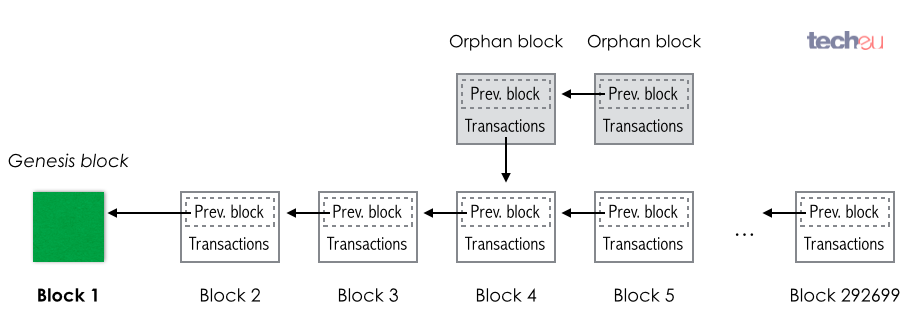
\includegraphics[width=10cm, height=6cm]{orphan.png}
\end{center}
Say Alice pays Bob, and an honest node broadcasts this. Bob accepts that he's been paid. Alice then
gets to broadcast her own transaction. She then makes a block with the \emph{prevBlock} hash as the one before her payment to Bob.
one of these blocks will be accepted. 
\section*{Incentives: Solves 3}
\begin{itemize}
  \item Can't penalize, but can reward nodes for working correctly.
    \begin{itemize}
      \item \emph{Incentive 1}: Block Reward (25 BTC, halves every 4 years). (Solves 3)
        \subitem 21 million max - block reward is how new coins are created; run out in 2140.
      \item \emph{Incentive 2}: Transaction Fee
        \subitem Incentive to have your transaction verified
      \item Remaining problems: 
        \subitem How to pick random node
        \subitem How to avoid free-for-all rewards
    \end{itemize}
  \item The miner gains if reward $>$ cost
    \subitem reward = block reward + tx fees
    \subitem mining cost = hardware cost + operating costs
  \item Aspects of decentralization in Bitcoin
    \begin{itemize}
      \item Peer to peer network, open to anyone, low barrier for entry
      \item Mining is open to everyone
      \item Updates to software - core developers trusted by the community who have a lot of power (Solve Problem 4)
    \end{itemize}
  \item New Problems from being Decentralized and Attacks:
    \begin{itemize}
      \item Blocks have a tendency to extend the block they hear about first
      \item Orphan Block
      \item Latency, not all nodes connected, internet connection, malicious nodes
      \item Attacks:
      \item Stealing - even if Alice gets to decide the next block, she can't steal because she has to create
        a valid transaction; can't forge signatures
      \item Denial of Service - even if Alice never validates Bob's transactions, an honest node will eventually do so.
      \item Sybil attack
        \subitem Can't gain more power by having more accounts
        \subitem Satoshi's original paper had 1 cpu = 1 vote
      \item Zero-confirmation transaction
        \subitem Bob gives Alice product before transaction has been verified
        \subitem 6 blocks; double spend probability goes down exponentially
        \subitem Never a 100\% guarantee
    \end{itemize}
  \item Solves the problem of not trusting a central authority - Problem 4
  \item 51\% attacker
    \begin{enumerate}
      \item CANNOT change block reward
      \item CANNOT spend other people's Bitcoin
      \item CANNOT change number of coins generated per block
      \item Suppress transactions
      \item Destroy confidence in Bitcoin
    \end{enumerate}
\end{itemize}


\section*{Changing the rules}
\begin{itemize}
  \item Two types of changes - soft forks; hard forks
    \subitem Soft forks are forward compatible; new rules are subset of old rules. Only applied if over 51\% agree.
    \subitem Hard forks are backward compatible; old rules are subset of new rules. Everyone needs to upgrade to new.
\end{itemize}



Source: \url{http://people.dsv.su.se/~matei/courses/IK2001_SJE/Chaum90.pdf}\\
Source: \url{http://blog.koehntopp.de/uploads/Chaum.BlindSigForPayment.1982.PDF}

\end{document}
